%!TEX root=./pfc.tex
\chapter[Ejemplos de uso]{\label{}
Ejemplos de uso}

A continuación se van a describir dos ejemplos para comprobar la potencia del sistema y conocer mejor su uso. 

\vspace{1cm}

\section{Ejemplo 1. Práctica de grupos.}

Este ejemplo se basará en crear una Wikicode de grupos, con dos usuarios por grupo previamente creados en el curso, y comprobar como el administrador/profesor puede ver de modo fácil sus estadísticas y código.

Esto será útil para prácticas grupales de Programación, y del mismo modo la interfaz será exactamente igual a la creada para prácticas individuales. Por lo que este ejemplo también será válido para dicho caso.

\newpage

\subsection{Creación}

\begin{itemize}
	\item Paso 1. Creación de la Wikicode. Seleccionamos las opciones necesarias para crear una Wikicode grupal.
\end{itemize}

\begin{figure}[h]
	\label{fig:ej1create}
	\includegraphics[width=\textwidth]{./img/ej1create.eps}
	\caption{Ejemplo 1. Creación de la Wikicode.}
\end{figure}

\newpage

\begin{itemize}
	\item Paso 2. El usuario desde su ventana principal del curso accederá a la Wikicode. No existe ningún tipo de diferencia con otra Wikicode.
\end{itemize}

\begin{figure}[h]
	\label{fig:ej1main}
	\includegraphics[width=\textwidth]{./img/ej1main.eps}
	\caption{Ejemplo 1. Ventana principal del usuario.}
\end{figure}

\newpage

\subsection{Interfaz de usuario}

A continuación se muestran las capturas de pantalla, una vez desarrollo el código por cualquiera de los usuarios que componen el grupo, que verían los componentes del \textbf{Grupo A}.

\begin{center}

\begin{figure}[h]
	\label{fig:ej1view1}
	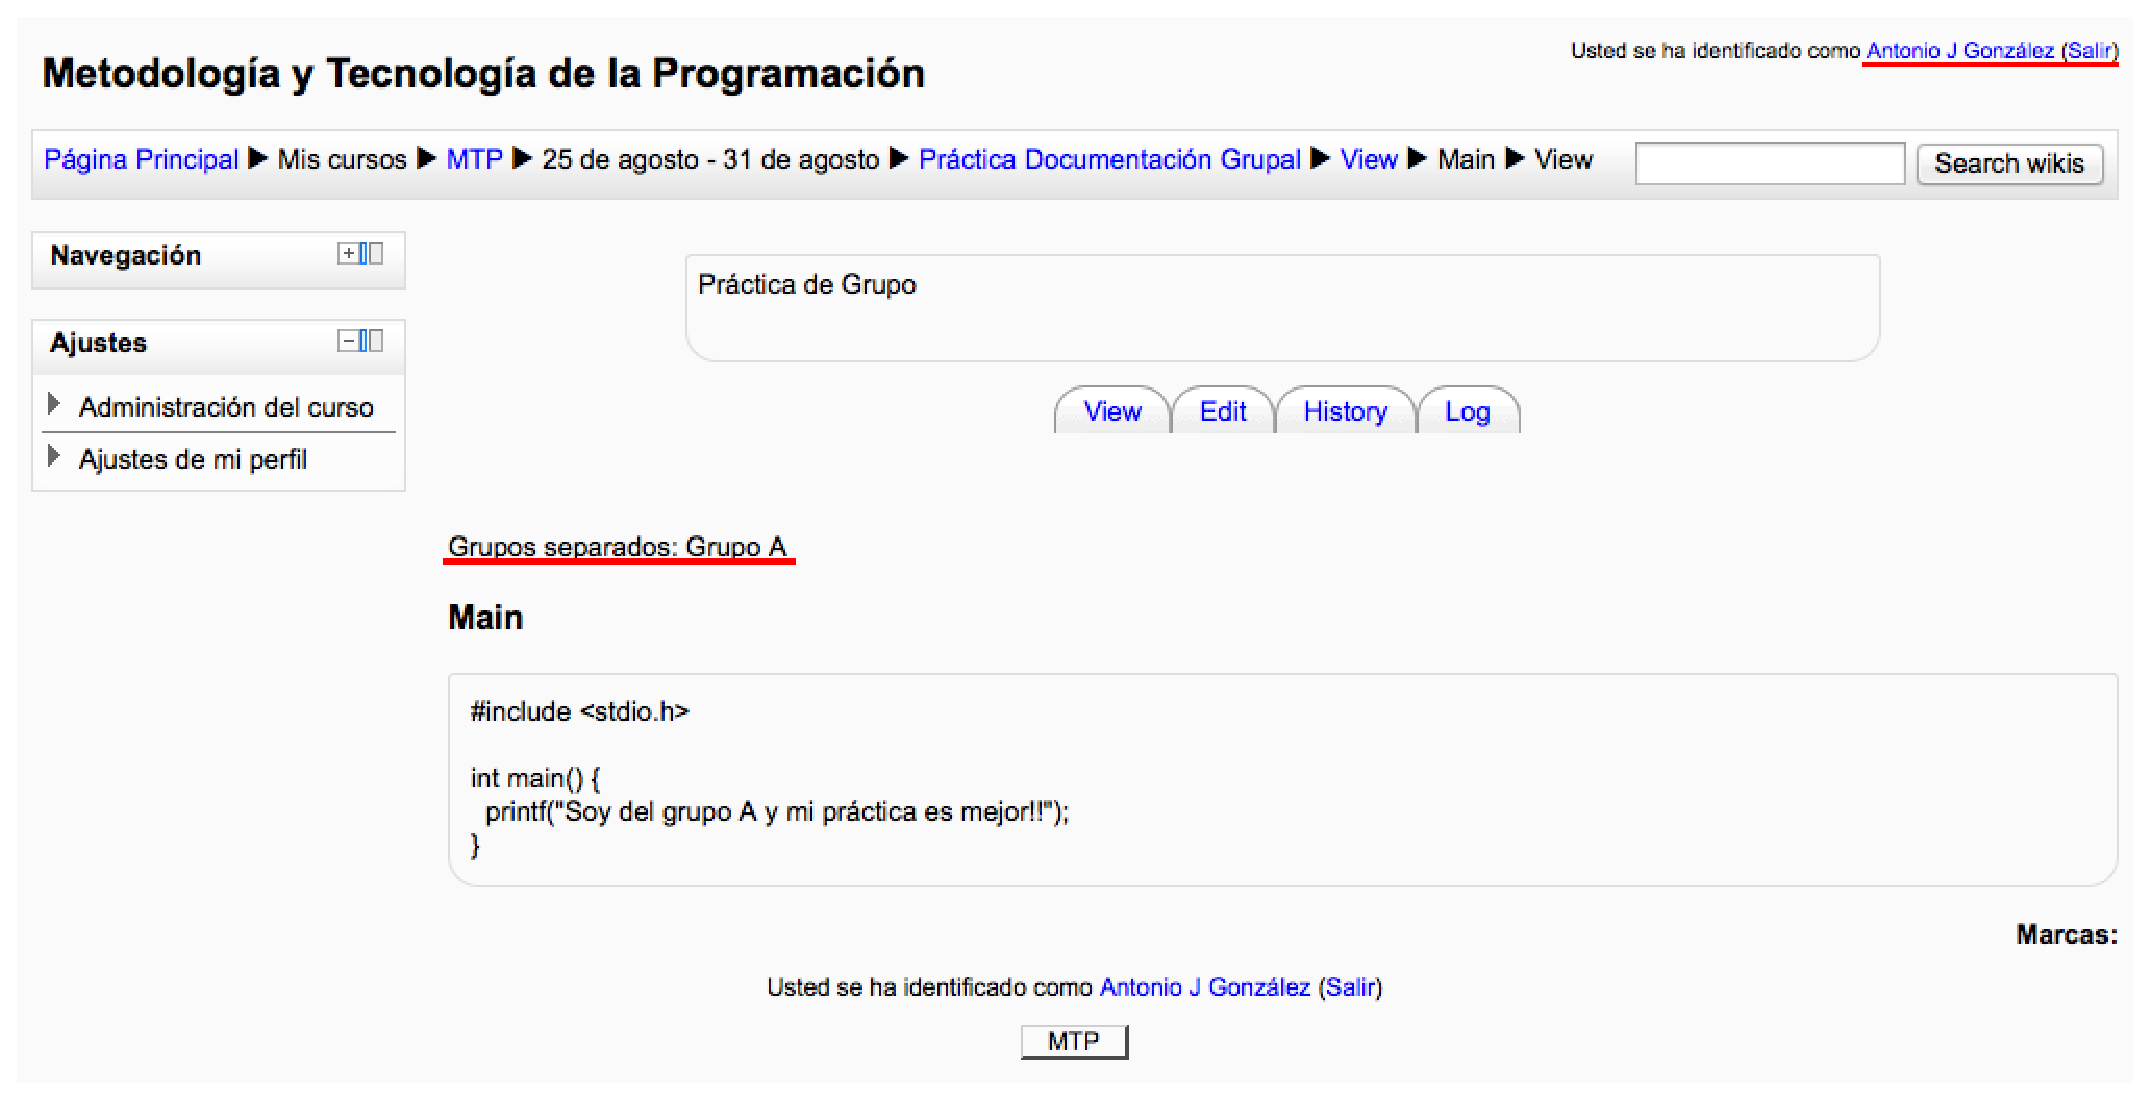
\includegraphics[scale=0.40]{./img/ej1view1.eps}
	\caption{Ejemplo 1. Pestaña view de la Wikicode. Usuario i32golea (Grupo A).}
\end{figure}

\begin{figure}[h]
	\label{fig:ej1view2}
	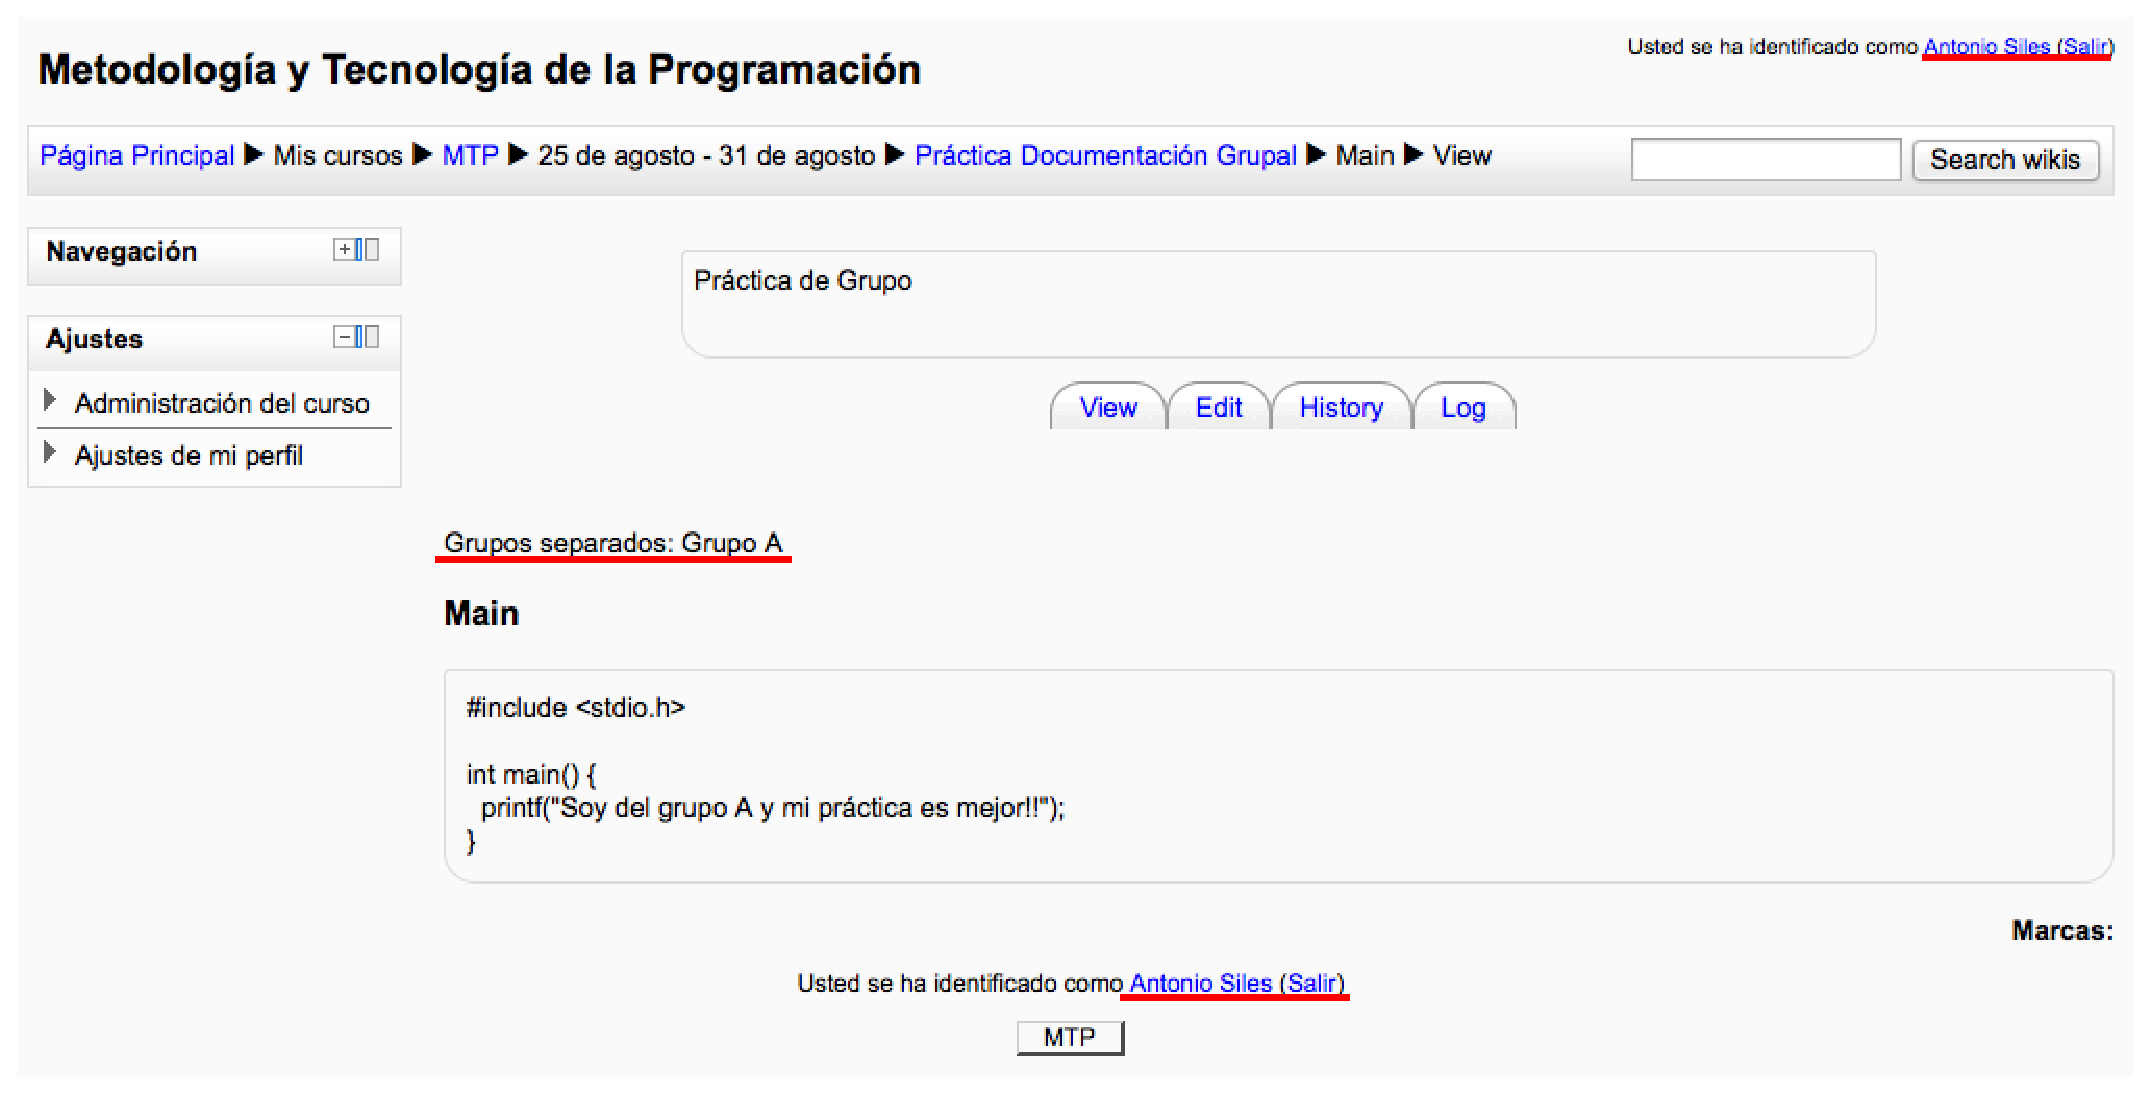
\includegraphics[scale=0.40]{./img/ej1view2.eps}
	\caption{Ejemplo 1. Pestaña view de la Wikicode. Usuario i32sibaa (Grupo A).}
\end{figure}

\end{center}

\newpage

Del mismo modo, esta sería la ventana que vería un componente cualquiera del \textbf{Grupo B}.

\begin{figure}[h]
	\label{fig:ej1view3}
	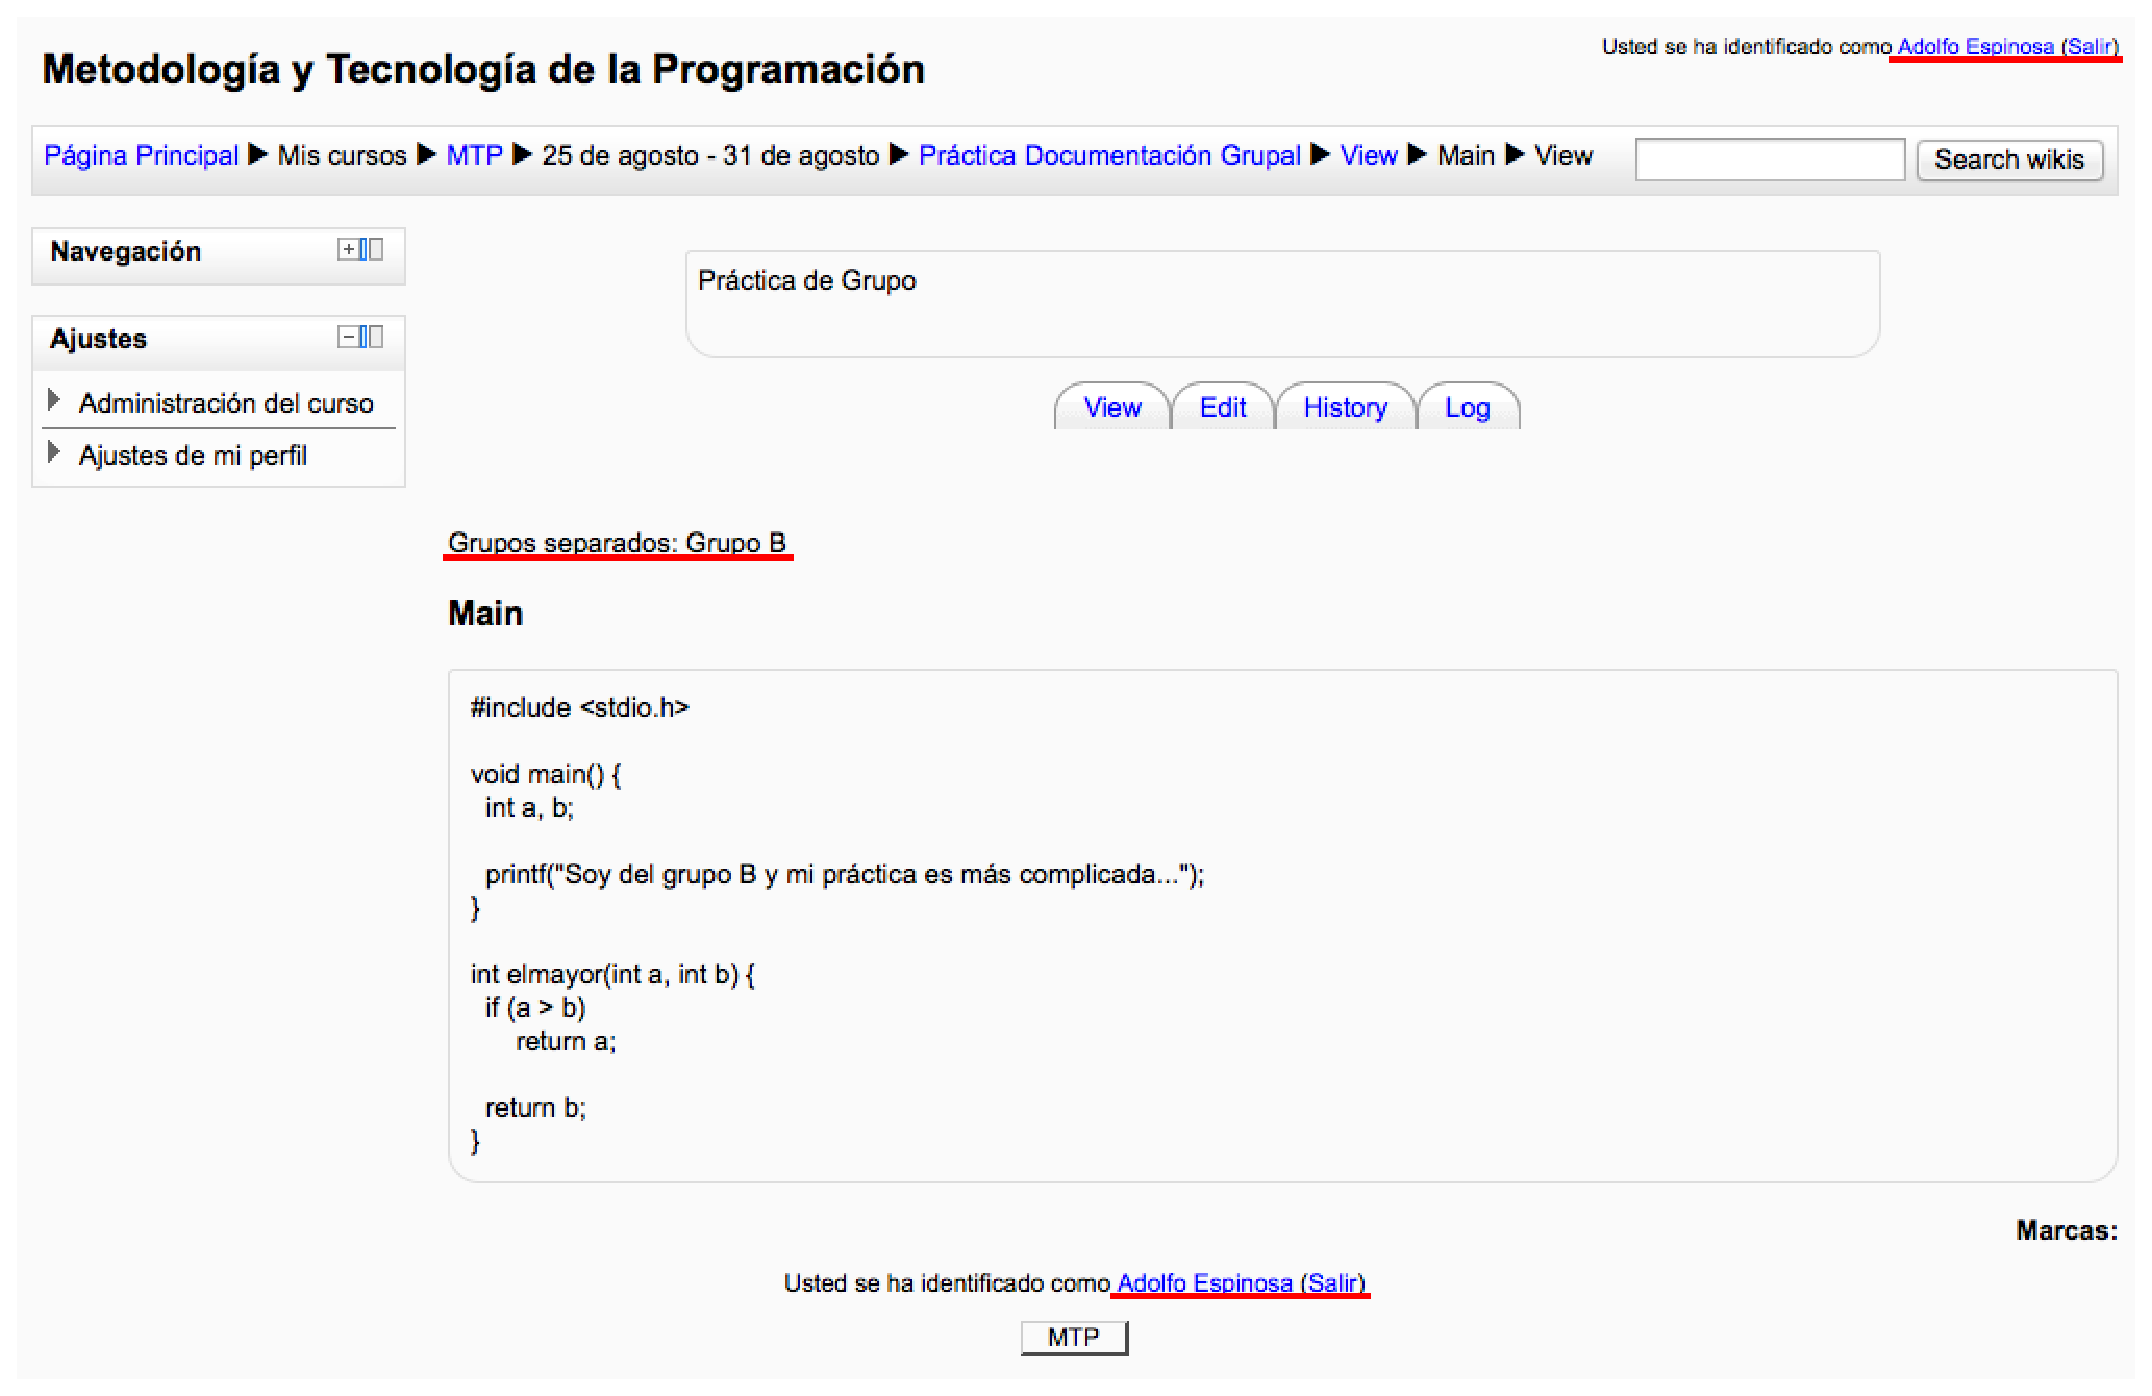
\includegraphics[width=\textwidth]{./img/ej1view3.eps}
	\caption{Ejemplo 1. Pestaña view de la Wikicode. Usuario i32esvaa (Grupo B).}
\end{figure}

Como podemos comprobar, para estos usuarios el hecho de que la Wikicode pertenezca o no a algún grupo es totalmente indiferente, y podrán acceder a todas las funcionalidades como si de una Wikicode individual o común para todos fuera. La única diferencia esgrime en los compañeros con los que desarrollarán el código.

\newpage

\subsection{Interfaz de profesor}

El profesor, sin embargo, una vez acceda a la Wikicode desde la pantalla principal del curso podrá seleccionar el grupo que desea ver.

\begin{figure}[h]
	\label{fig:ej1admin}
	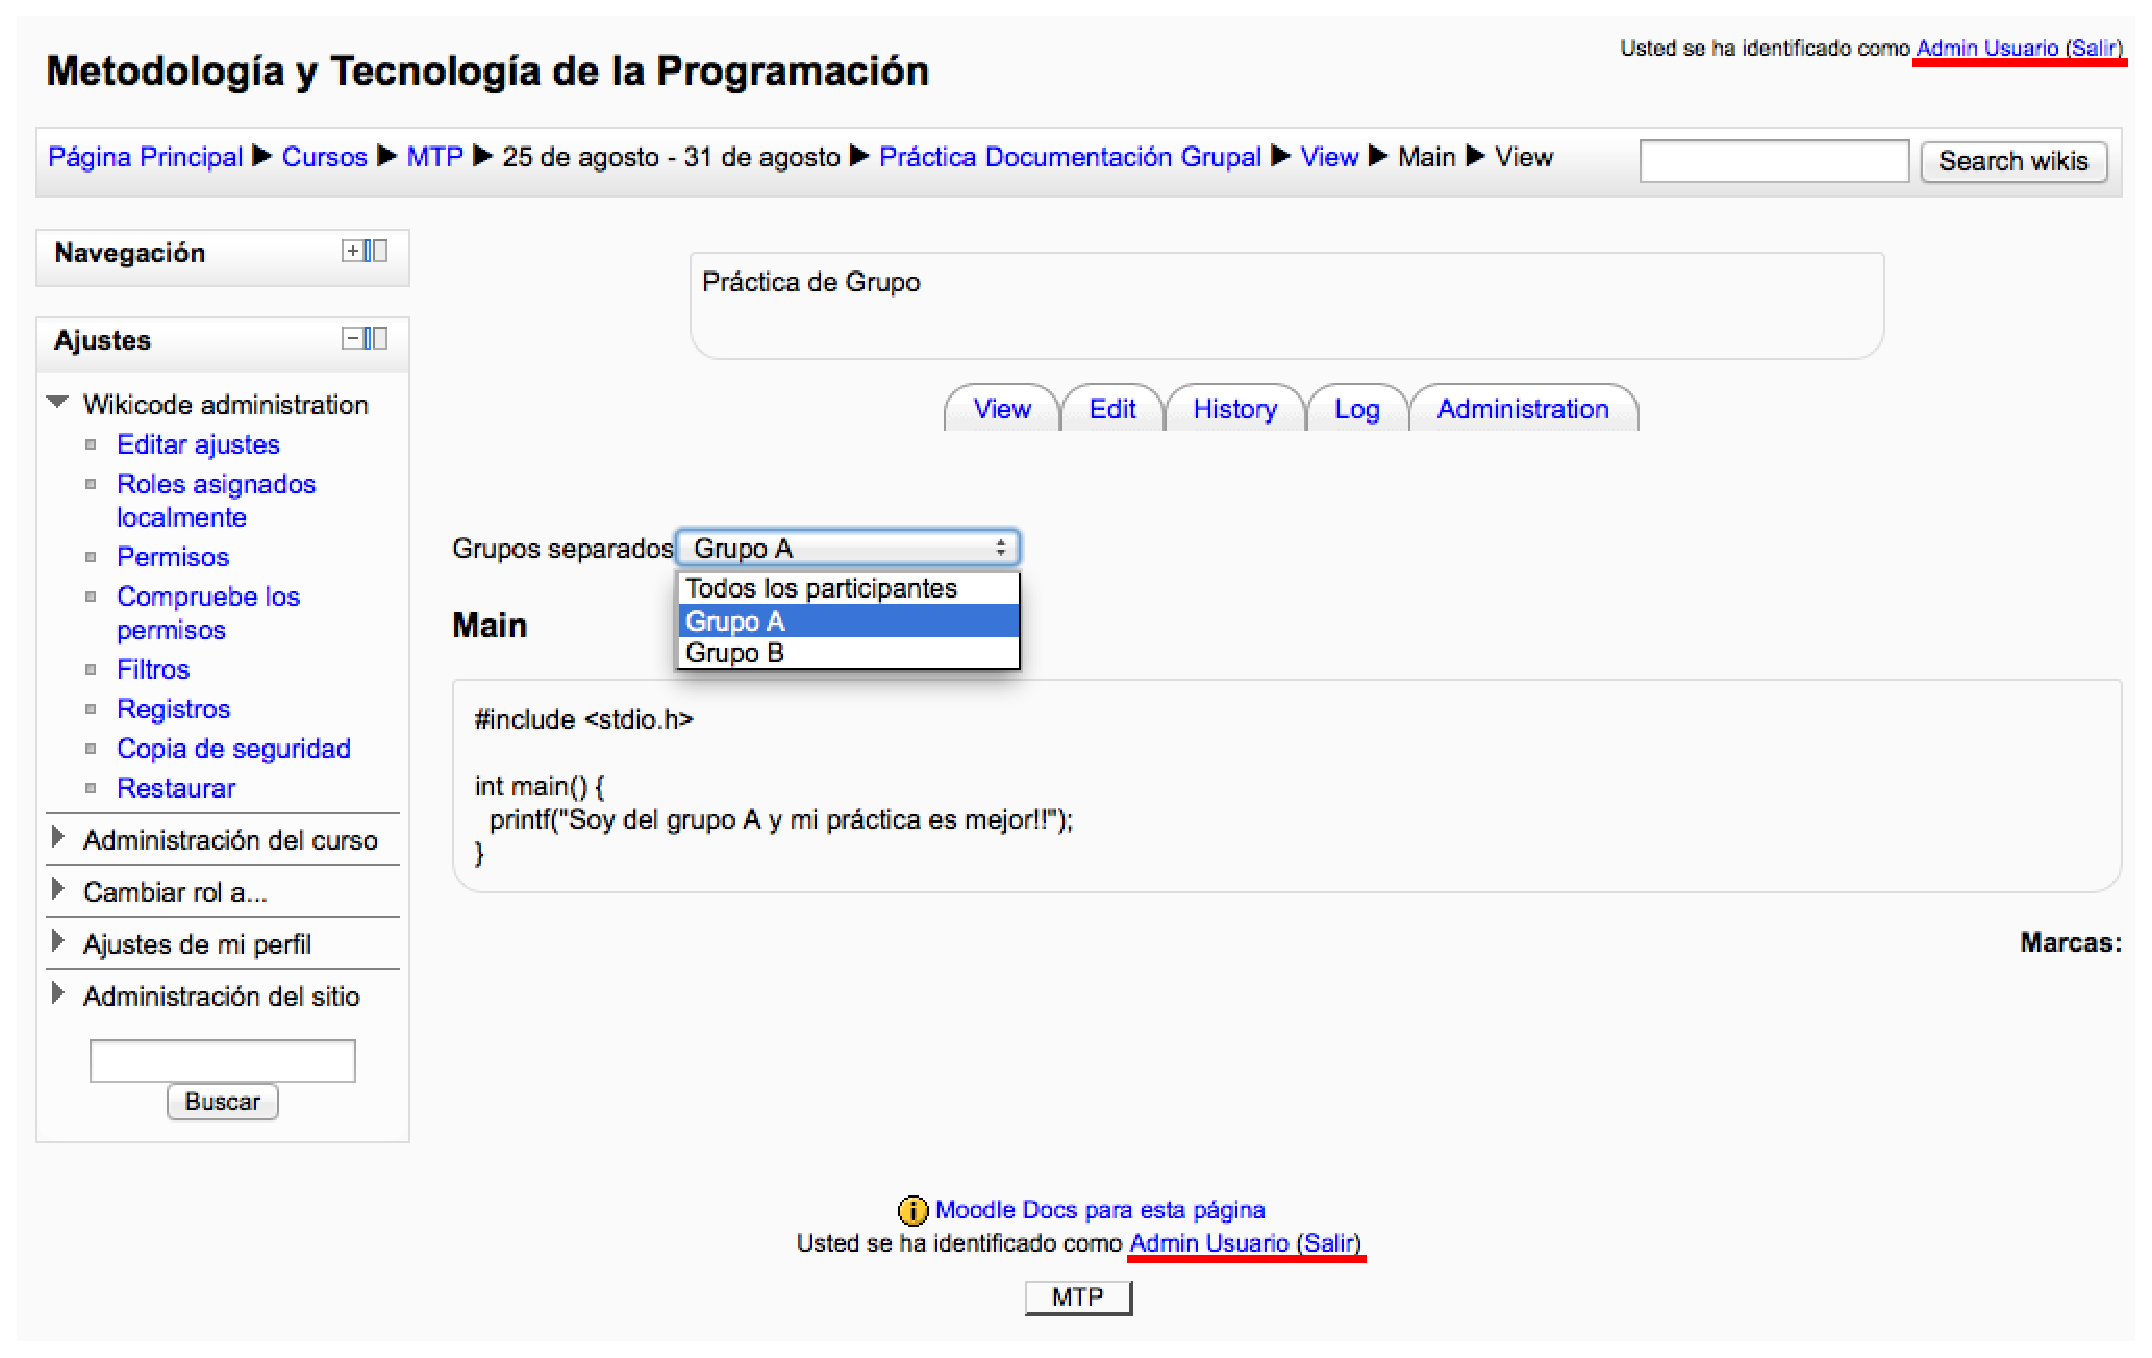
\includegraphics[width=\textwidth]{./img/ej1admin.eps}
	\caption{Ejemplo 1. Pestaña view del profesor.}
\end{figure}

\newpage

Una vez tenga seleccionada la que desee, podrá navegar por sus opciones.

\begin{figure}[h]
	\label{fig:ej1log}
	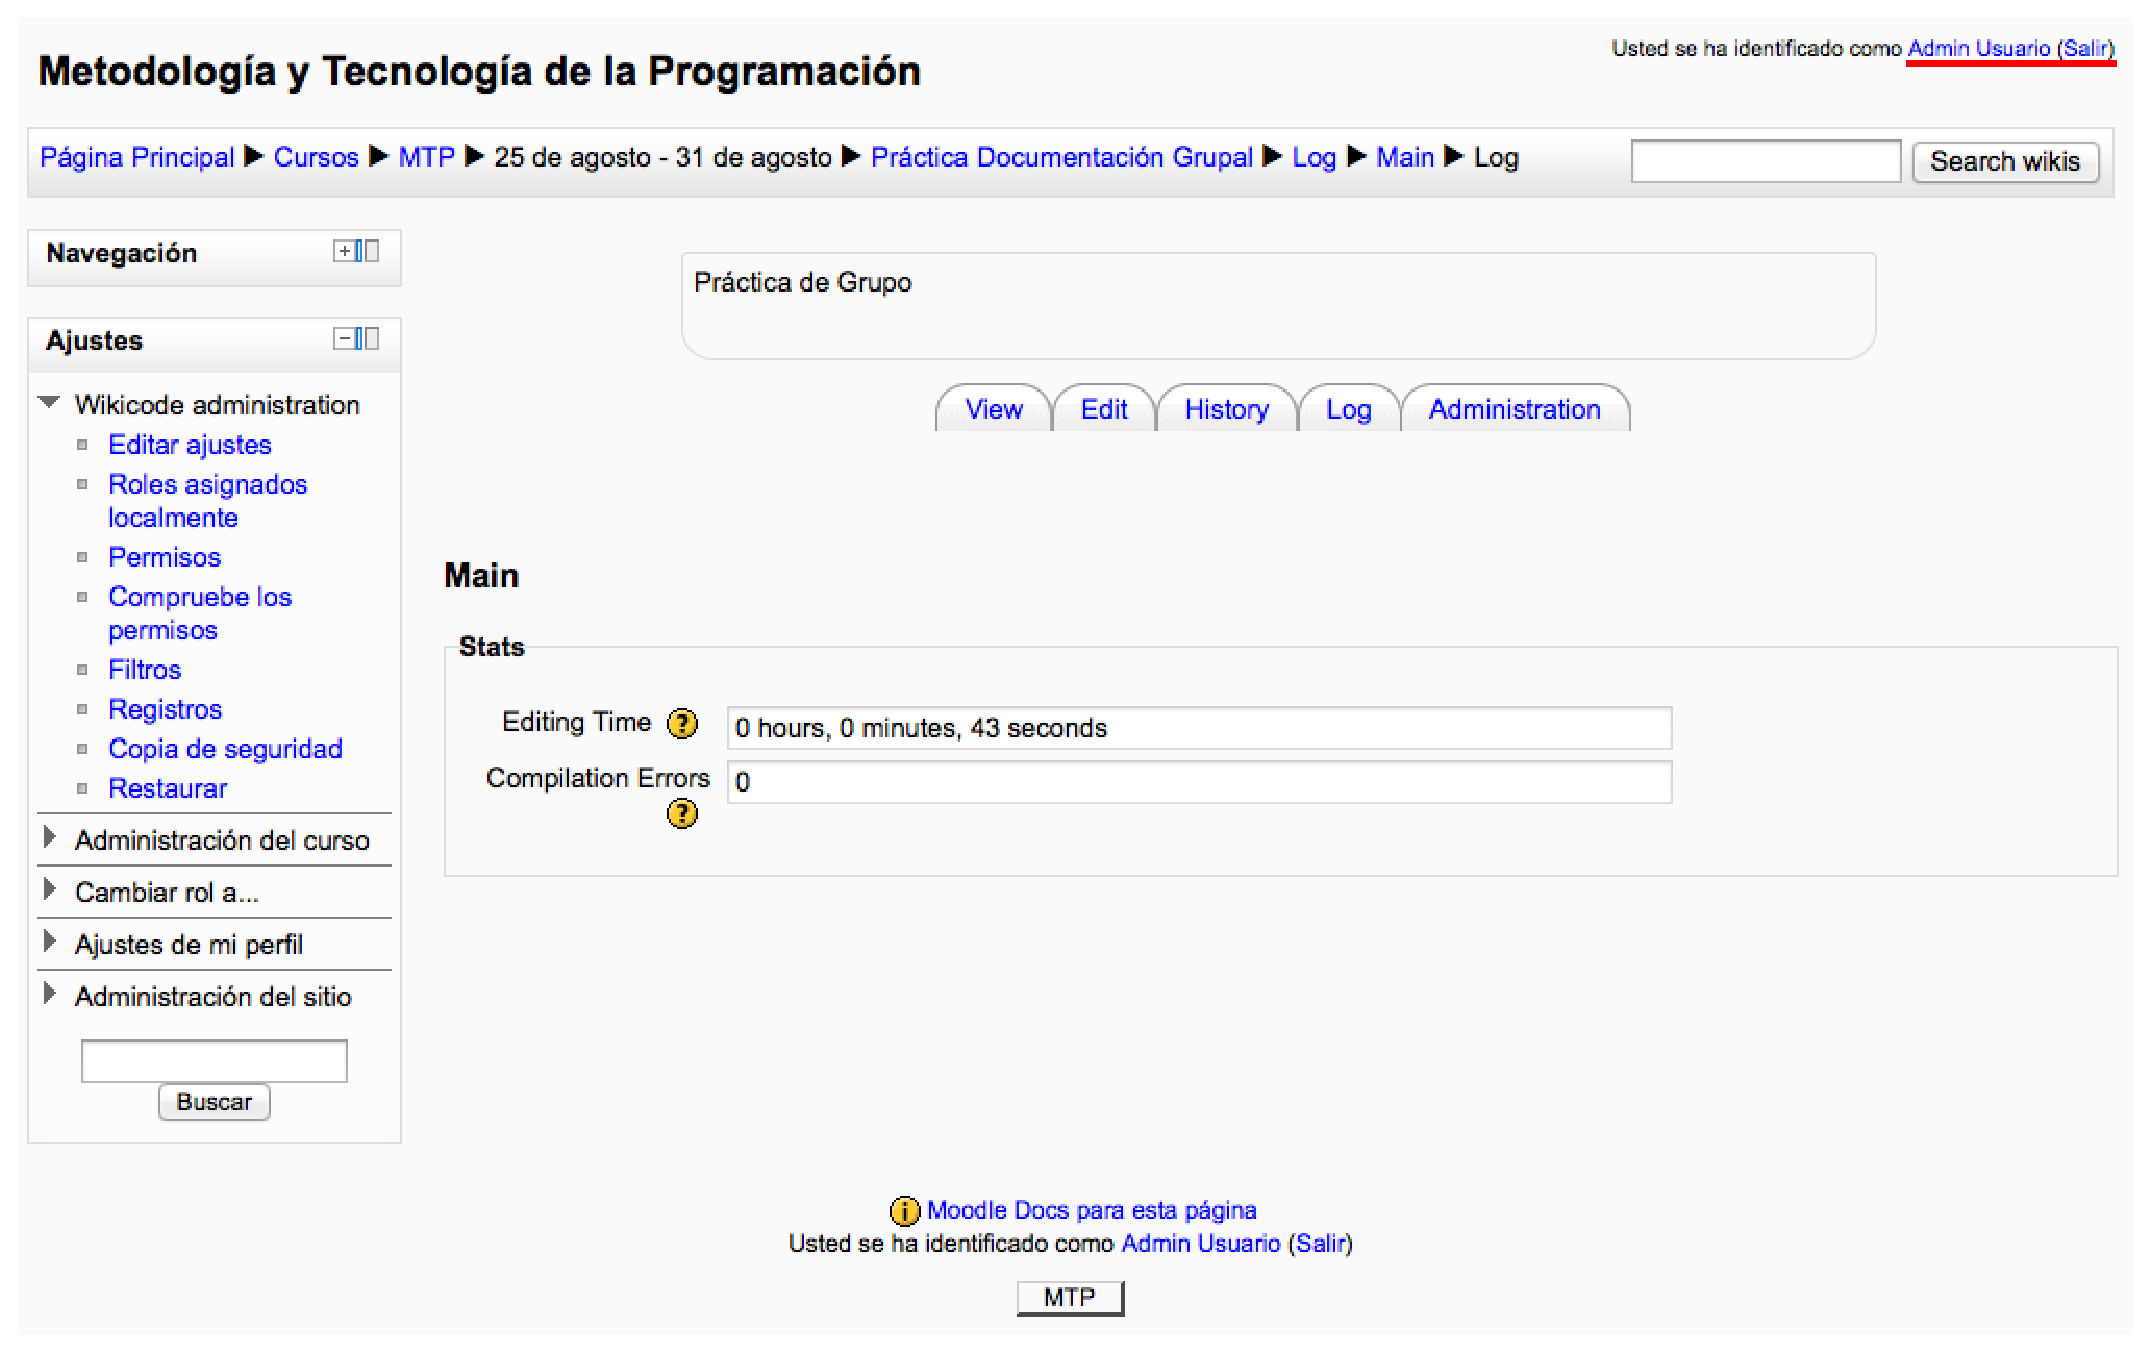
\includegraphics[width=\textwidth]{./img/ej1log.eps}
	\caption{Ejemplo 1. Pestaña log seleccionada por el profesor.}
\end{figure}

\newpage

\subsection{Seguridad}

Si un usuario malintencionado intenta acceder a la Wikicode de otro grupo sin tener permisos para ello por métodos de \emph{SQL injection}\footnote{\textbf{SQL Injection:} Método de infiltración de código intruso que se vale de una vulnerabilidad informática presente en una aplicación en el nivel de validación de las entradas para realizar consultas a una base de datos.}, esta internamente comprobará las credenciales del usuario y evitará el acceso sin permiso.

\begin{figure}[h]
	\label{fig:ej1security}
	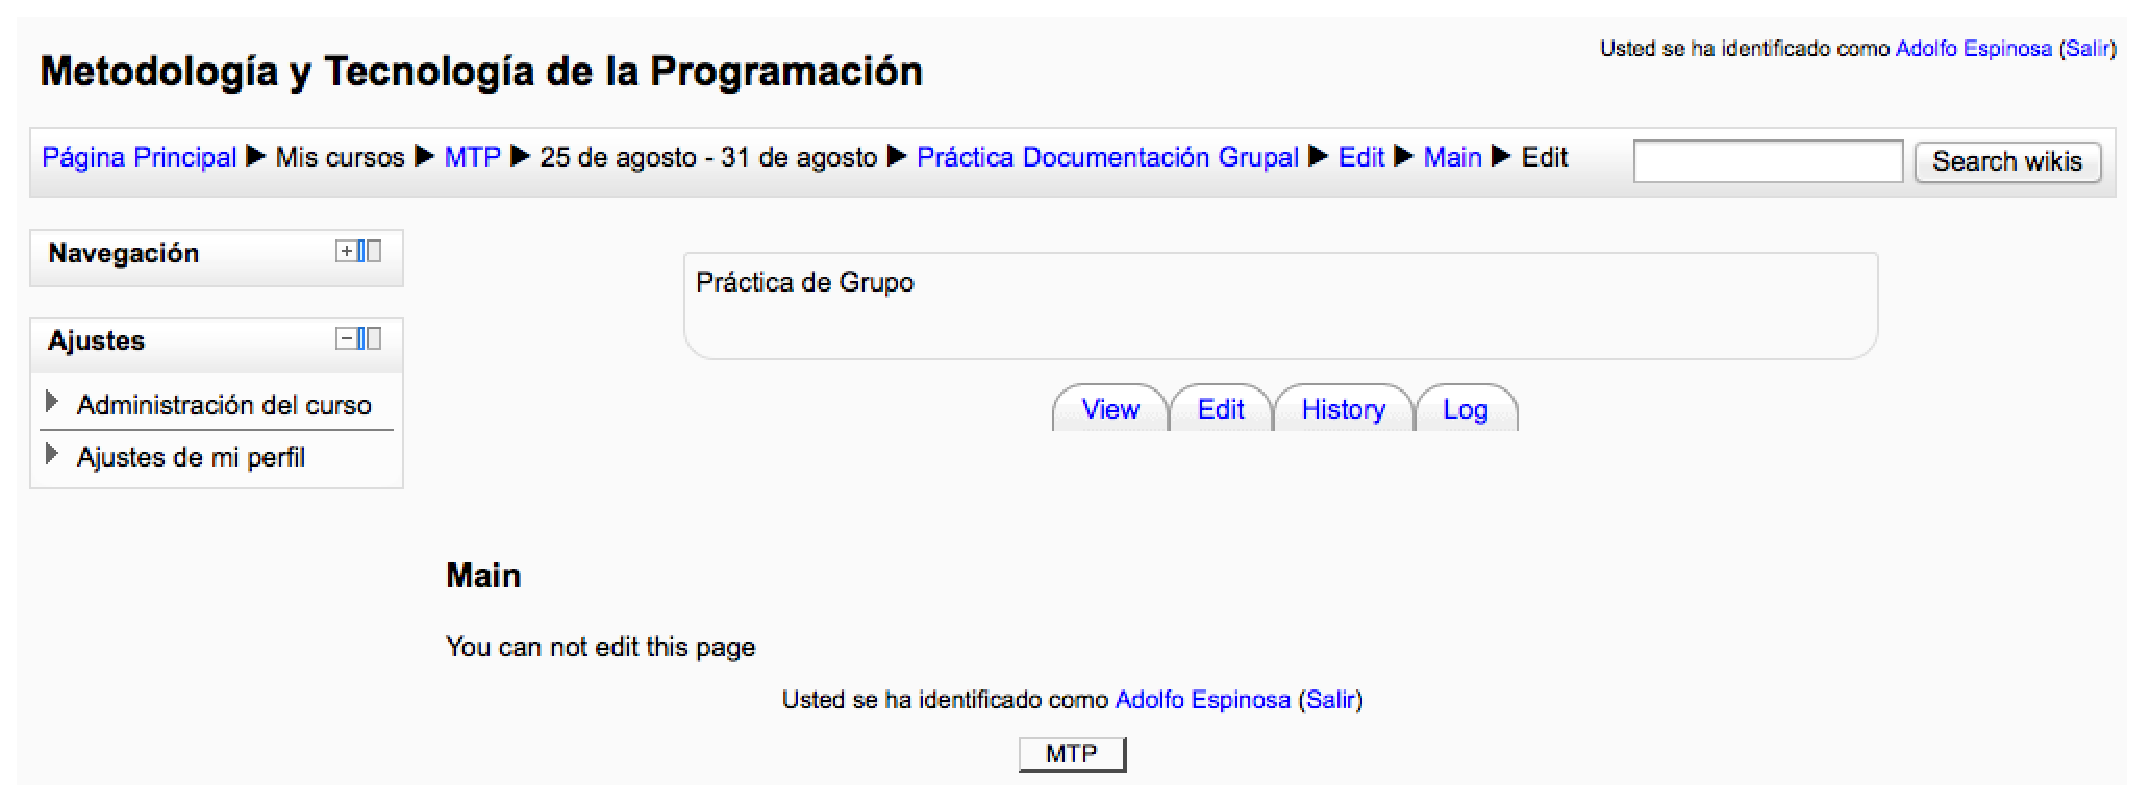
\includegraphics[width=\textwidth]{./img/ej1security.eps}
	\caption{Ejemplo 1. Acceso malintencionado no conseguido.}
\end{figure}

\newpage

\section{Ejemplo 2. Exclusión mutua.}

\let\thefootnote\relax\footnotetext{\textbf{Exclusión mutua:} Método usado en programación concurrente para evitar el uso simultáneo de recursos comunes por fragmentos de código conocidos como secciones críticas.}

En algunas ocasiones, y si los usuario de una Wikicode no se han comunicado con anterioridad, puede ocurrir que dos o más usuarios quieran modificar una misma función de modo paralelo. Como el refresco del editor no es automático, sino que se va actualizando a medida que se va escribiendo para mejorar rendimiento, puede ocurrir que un usuario intente modificar una función ya bloqueada por otro usuario y que aún no le haya sido notificada.

Como podemos ver a continuación, dos usuarios entran a modificar el código y ambos ven que la función \textbf{exclusion} está desbloqueada.

\begin{center}

\begin{figure}[h]
	\label{fig:ej1edit2}
	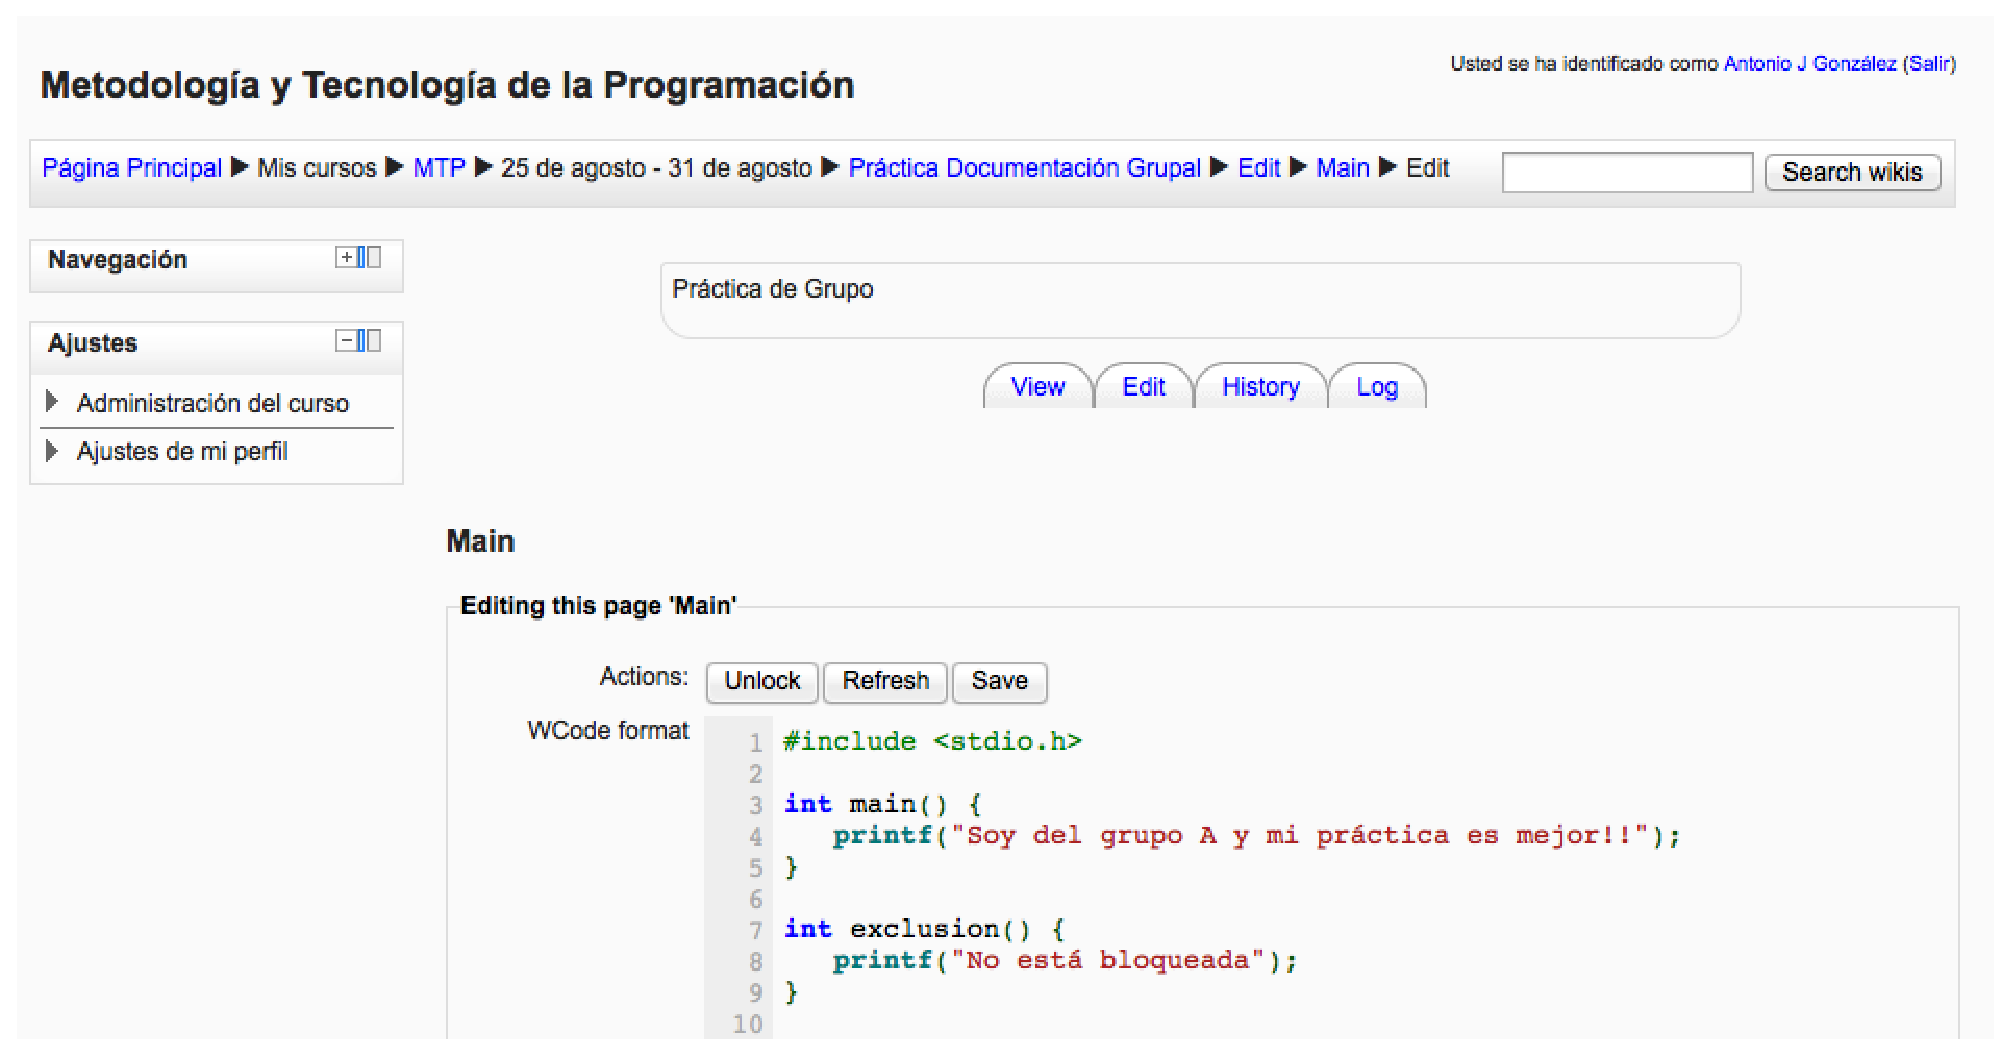
\includegraphics[scale=0.40]{./img/ej2edit2.eps}
	\caption{Ejemplo 2. Pestaña edit Wikicode. Usuario i32golea.}
\end{figure}

\begin{figure}[h]
	\label{fig:ej1edit1}
	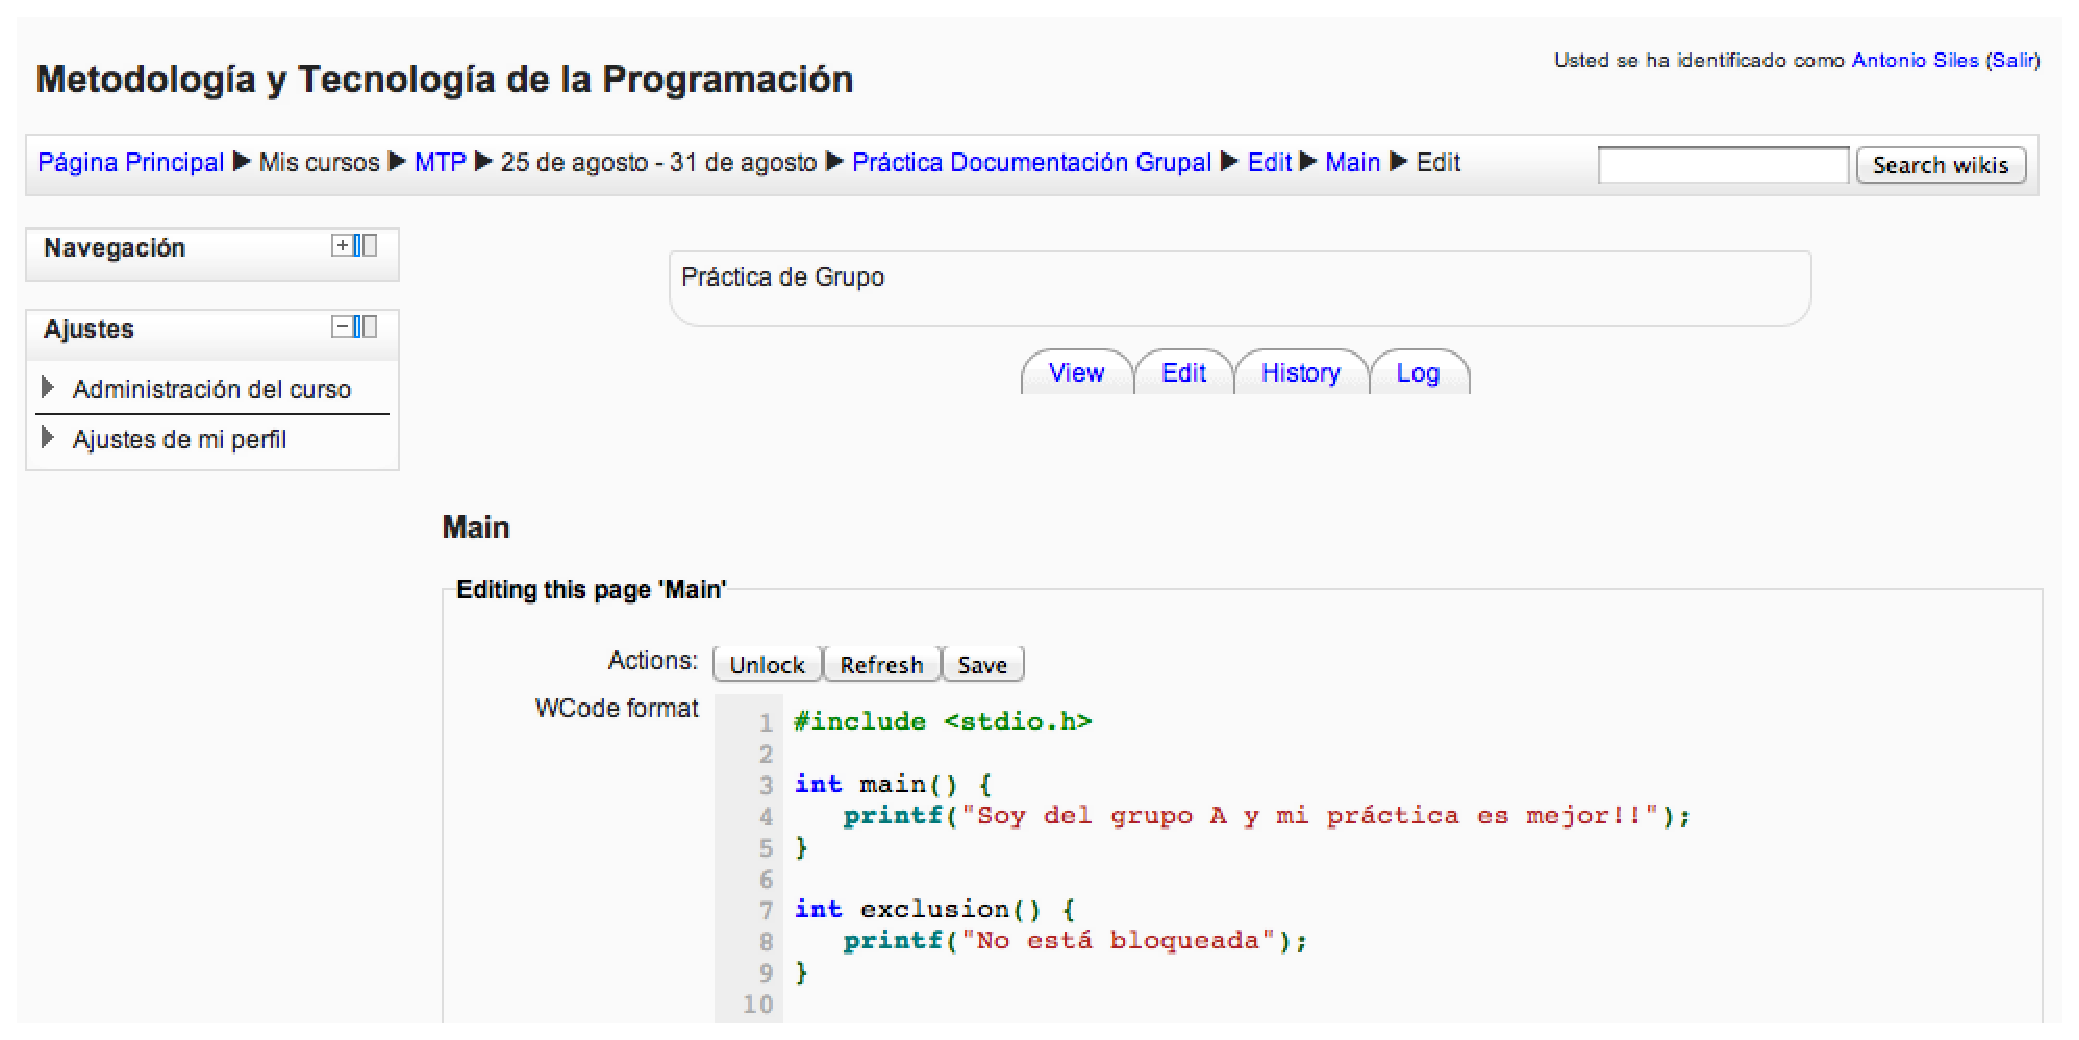
\includegraphics[scale=0.40]{./img/ej2edit1.eps}
	\caption{Ejemplo 2. Pestaña edit Wikicode. Usuario i32sibaa.}
\end{figure}

\end{center}

\newpage

En ese momento ambos intentan modificar la función, pero en primer lugar lo hace el usuario \textbf{i32golea}.

\begin{figure}[h]
	\begin{center}
	\label{fig:ej1edit3}
	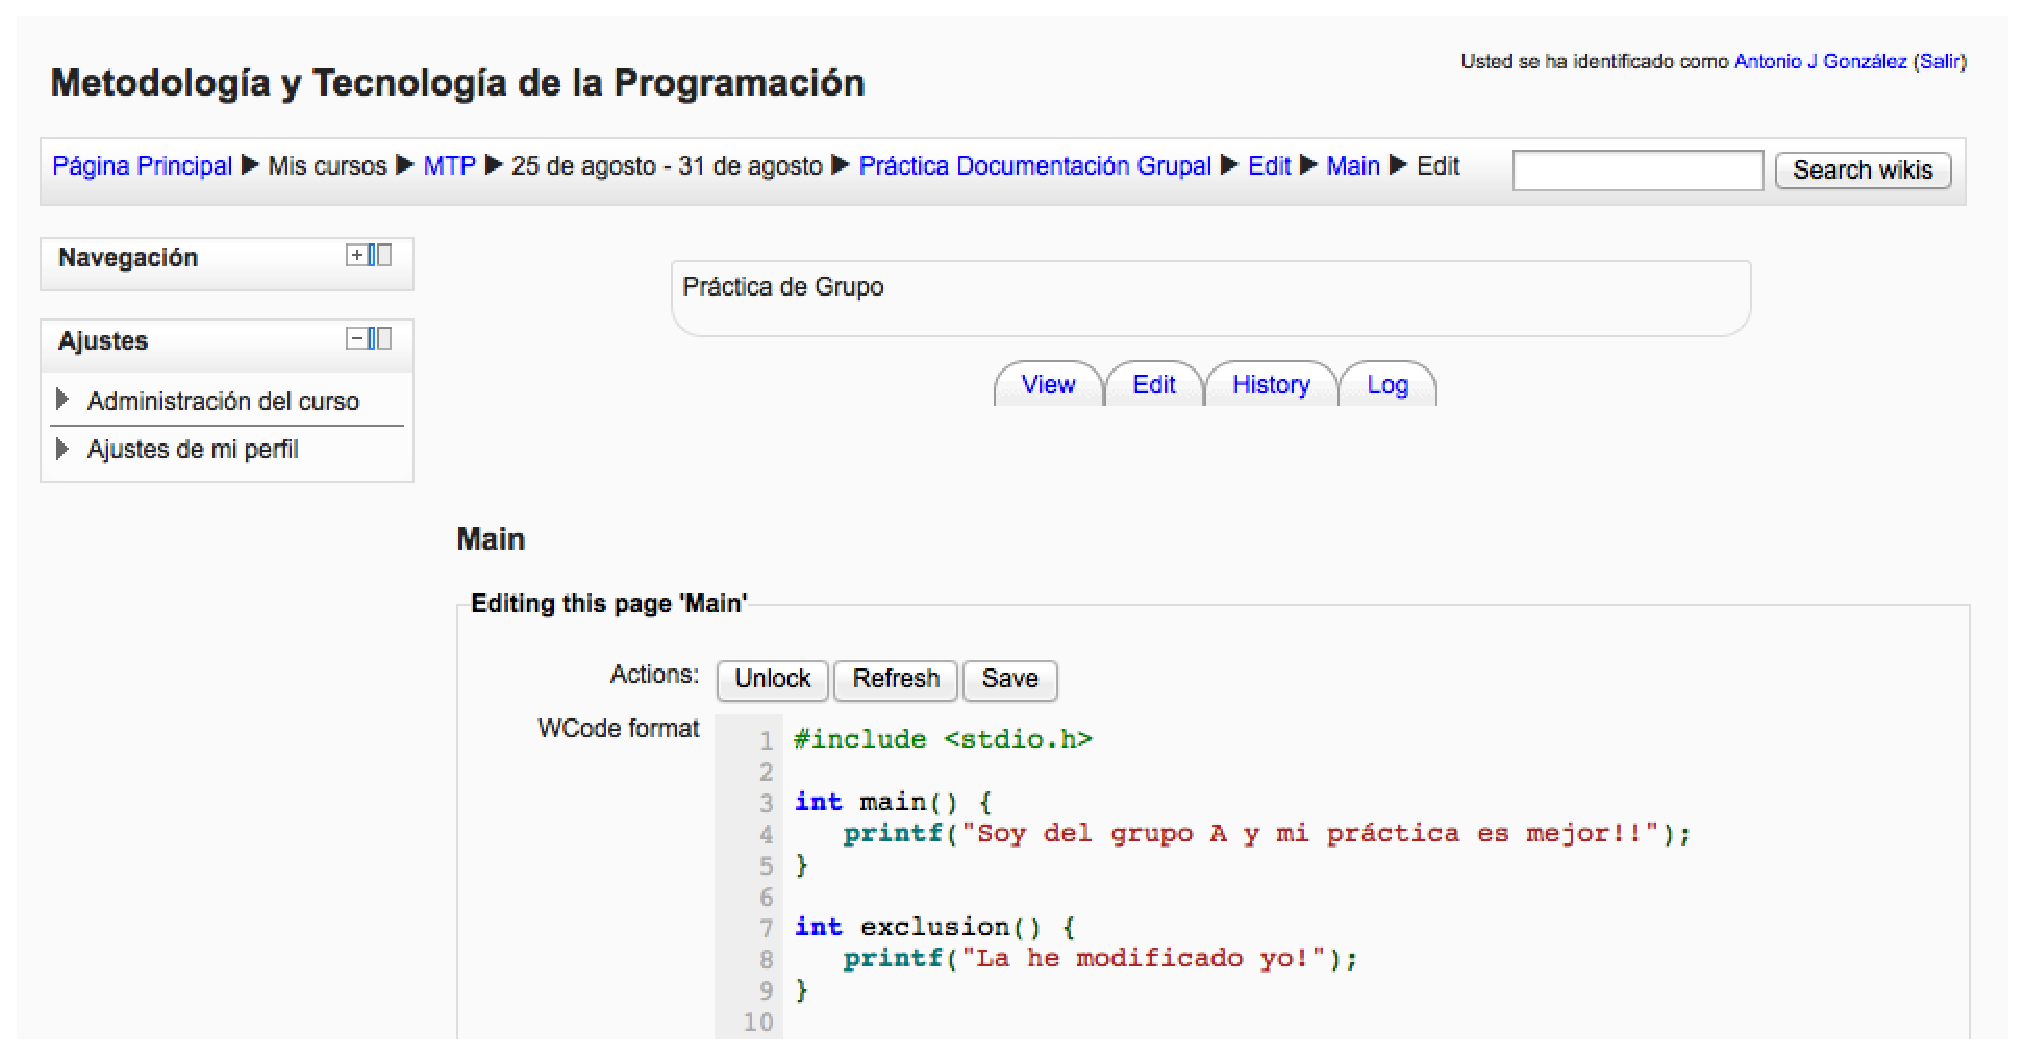
\includegraphics[scale=0.40]{./img/ej2edit3.eps}
	\caption{Ejemplo 2. Modificación función exclusion. Usuario i32golea.}
	\end{center}
\end{figure}

\newpage

Cuando el usuario \textbf{i32sibaa} proceda a modificar dicha función, y puesto que su actuación es posterior, el sistema no se lo permitirá y le notificará que la función ya ha sido bloqueada.

\begin{figure}[h]
	\begin{center}
	\label{fig:ej1edit4}
	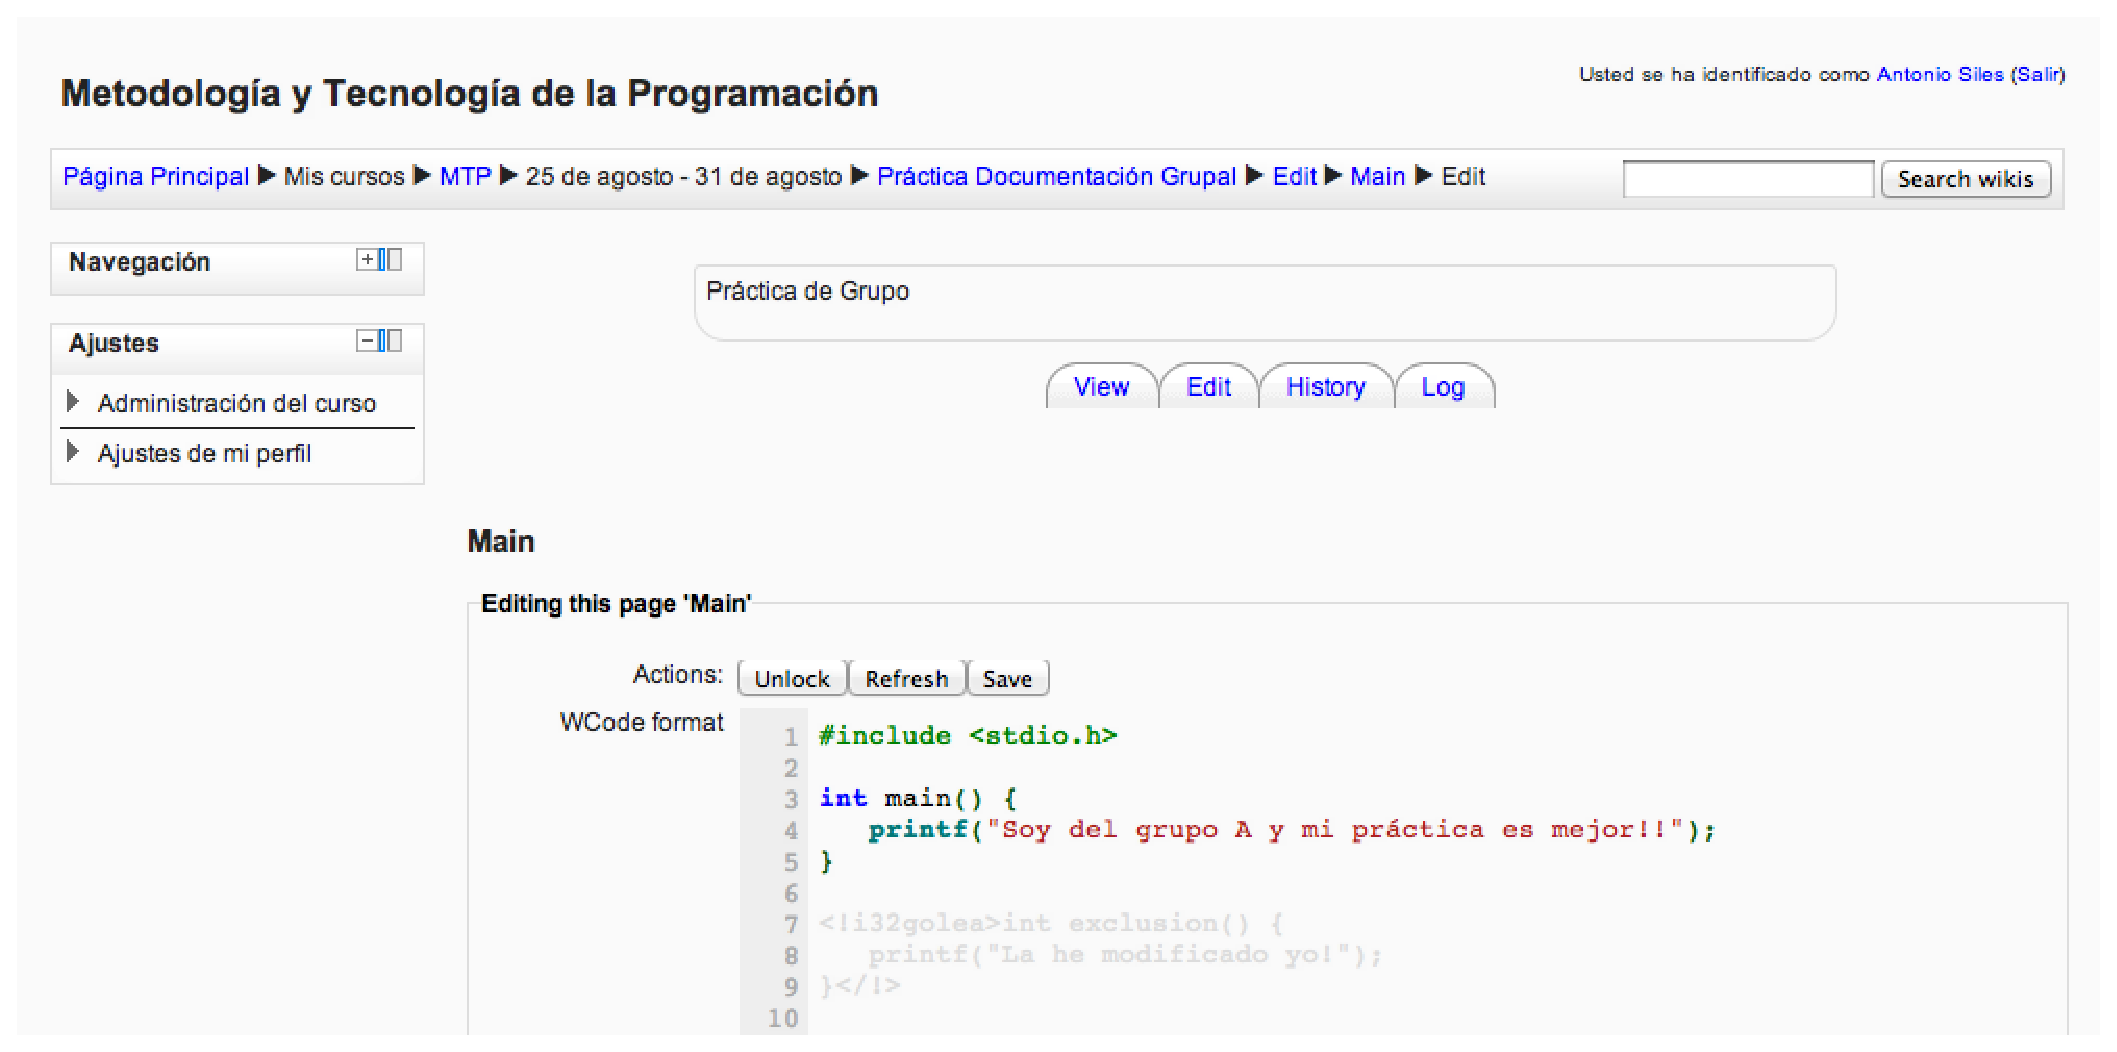
\includegraphics[scale=0.40]{./img/ej2edit4.eps}
	\caption{Ejemplo 2. Función bloqueada por el usuario i32golea. Interfaz de i32sibaa.}
	\end{center}
\end{figure}

A partir de ese momento y hasta que el usuario decida salvar la Wikicode o desbloquear la función, únicamente el usuario \textbf{i32golea} podrá modificar la función.































